\documentclass[twocolumn]{ctexart}
% ctexart、ctexrep、ctexbook和ctexbeamer, 对应 LaTeX 的article、report、book和beamer
\usepackage[a4paper,left=3cm,right=3cm,top=2.6cm,bottom=2.6cm]{geometry} % 设置页面尺寸
\usepackage{fancyhdr} % 设置页眉页边页脚
\usepackage{multicol} % 多栏排版
\usepackage{xeCJK} % 中文支持
\usepackage{ctex} % 中文支持
\usepackage{footmisc} % 控制脚注格式,包括编号、字体、分隔线等
\usepackage{titletoc} % 定制目录列表样式
\usepackage{fontspec} % XeTeX下的字体选择宏包
\usepackage{setspace} % 行距
\usepackage{graphicx} % 插图
\usepackage{pdfpages} % 引用pdf页面
\usepackage{booktabs} % 三线表
\usepackage{multirow} % 表格多行支持
\usepackage{caption} % figure和table等中的说明文字
\usepackage{tikz} % 绘图
\usepackage{etoolbox} % 给宏包打补丁
\usepackage{hyperref} % 超链接
\usepackage{xcolor} % 颜色支持
\usepackage{array} % 数学表格
\usepackage{amsmath} % 数学公式
\usepackage{amssymb} % 数学字体与符号
\usepackage{amsthm} % 数学定理格式
\usepackage{subfig} % 排版子图
\usepackage{float} % 浮动体格式控制
\usepackage{lmodern} % 一种字体支持
\usepackage{listings} % 插入代码
\usepackage{tcolorbox} % 好看的块环境
\usepackage{pifont} % 字体支持
\usepackage{perpage} %the perpage package
\usepackage{mathdesign} % some math fonts
\usepackage{ulem} %一些文字强调的宏包
\usepackage{fancyvrb} % some fancy verbatim 
\usepackage{enumitem} % 列表项目
\usepackage{txfonts} % 一些字体
\usepackage{makecell}
\usepackage{mathrsfs}
\usepackage{subfig}                 % 子图包,不要与{subfigure}混用,{subfig}较新
\usepackage{overpic}   
%重置每页脚注序号
\pagestyle{headings}
\MakePerPage{footnote} %the perpage package command
\renewcommand \thefootnote{\ding{\numexpr171+\value{footnote}}}
% 为tcolorbox导入三个程序包
\tcbuselibrary{skins, breakable, theorems} 

% 设置代码格式 - 关键字加粗, 其余为正常。非彩色
\lstset{
    aboveskip=5mm,
    belowskip=5mm,
    breaklines=true,
    breakatwhitespace=true,
    columns=flexible,
    extendedchars=false,
    showstringspaces=false,
    numbers=none,
    basicstyle={\small\ttfamily},
    captionpos=t,
    frame=tb,
    tabsize=4
}

\lstdefinestyle{cpp} {
  language=C++
}

\lstdefinestyle{c++} {
  language=C++
}

\lstdefinestyle{python} {
  language=python,
  morekeywords={as}
}


% 为目录添加 PDF 链接
\addtocontents{toc}{\protect\hypersetup{hidelinks}}

% 设置「目录」二字格式
\renewcommand{\contentsname}{
  \fontsize{16pt}{\baselineskip}
  \normalfont\heiti{目~~~~录}
  \vspace{-8pt}
}

% 定理、定义、证明
\newtheorem{theorem}{定理}[section]
\newtheorem{definition}{定义}[section]
\newtheorem{lemma}{引理}[section]
\newtheorem{corollary}{推论}[section]
\newtheorem{example}{例}
\newtheorem{proposition}{命题}[section]

\title{电动力学考前复习及习题练习}
\author{洛白}
\date{\today}

\begin{document}

% 显示标题作者时间
\maketitle
\newpage

% 调整目录行间距
\renewcommand{\baselinestretch}{1.35}
% 添加目录
\tableofcontents
\newpage

% 正文 22 磅的行距
\setlength{\parskip}{0em}
\renewcommand{\baselinestretch}{1.53}


\section{矢量基础}
% \subsection{置换符号Ricci里奇}
\begin{align}
  \bigtriangledown=\frac{\partial }{\partial x}e_x+\frac{\partial }{\partial y}e_y+\frac{\partial }{\partial z}e_z  
  \tag{1.1.a} \\
  \Delta=\bigtriangledown \cdot \bigtriangledown=\frac{\partial^2 }{\partial x^2}+\frac{\partial^2 }{\partial y^2}+\frac{\partial^2 }{\partial z^2}
  \tag{1.1.b} 
\end{align}
\subsection{向量表示}

\subsection{标量场}
\subsubsection{梯度$\bigtriangledown f$}
\begin{definition}[方向导数]
标量函数$f$ 沿着某一个方向变化的速率,可以记作$grad \mathrm{f}\cdot \vec{e}$
\end{definition}
最大的方向导数我们叫做\textbf{梯度},记作$grad \mathrm{f}\equiv \bigtriangledown \mathrm{f}=(\frac{\partial }{\partial x}e_x+\frac{\partial }{\partial y}e_y+\frac{\partial }{\partial z}e_z )f $
\begin{definition}[等值面]
$$
u(x,y,z)=c
$$
\subsection{矢量场}
\begin{definition}[矢量线]
它与$M$处$\mathrm{d}{r}$平行,对于如下函数
$$
\vec{A}(t)=A_xe_x+A_ye_y+A_ze_z
$$
有 $$\frac{\mathrm{d}{x}}{A_x}=\frac{\mathrm{d}{y}}{A_y}=\frac{\mathrm{d}{z}}{A_z}$$

\end{definition}
\end{definition}
\begin{definition}[通量]
对于一个矢量场$\vec{F}$,它穿过一个面元$\mathrm{d}{\sigma}$的通量为
\begin{equation}
\mathrm{d}\psi=\vec{F} \mathrm{d}{\sigma} e_n=\vec{F} \mathrm{d}{\sigma} \cos \theta \tag{1.2}
\end{equation} 
\end{definition}
\subsubsection{散度 div $\bigtriangledown \cdot \vec{A}$}
因为通量不能很好地反映曲面上某一点地发散性质,所以引入三度。
他表示空间某点单位体积的通量,设在闭合曲面S上,下面极限存在
\begin{equation}
%  \begin{aligned}
 \lim_{\Delta v \to 0} \frac{\int\mathrm{d}\psi}{\Delta v}=\Delta \cdot \vec{A}=(\frac{\partial A_x }{\partial x}+\frac{\partial A_y }{\partial y}+\frac{\partial A_z}{\partial z})   \tag{1.3}
%  \end{aligned}
\end{equation}
\subsubsection{环量和旋度$\bigtriangledown \times  \vec{A}$}
\begin{definition}[环量]
\begin{equation}
\oint_{l} F \cdot \mathrm{d}{\textbf{l}}=\oint_{l} F \cdot \mathrm{d}{{l}} \cos \theta  \tag{1.3}
\end{equation}
\end{definition}
\begin{equation}
rot \vec{A}=\lim_{\Delta S \to 0} \frac{\oint_{l} F \cdot \mathrm{d}{\textbf{l}}}{\Delta s}=\bigtriangledown \times \vec{A} \oint_{l} F \cdot \mathrm{d}{\textbf{l}}
\tag{1.4}
\end{equation}
\subsection{矢量微积分定理}
\begin{align}
 \tag{1.5.a} \\
\end{align}
\subsection{其他常用公式}
\subsubsection{矢量三重积}
\begin{align}
  A \times(B \times C)&=B(A \cdot C)-C(A \cdot B)  \tag{1.8.a} \\
  ( A \times B ) \times C &= - C \times ( A \times B ) = - A ( B \cdot C ) + B ( A \cdot C )  \tag{1.8.b} 
\end{align}
\subsubsection{标量三重积}
\begin{equation}
  A \cdot(B \times C)=B \cdot(C \times A)=C \cdot(A \times B) \tag{1.7}
\end{equation}
\subsubsection{运算规律}

\begin{align}
  grad \left[ f(u,v)\right]& = \frac{\partial f}{\partial u}gradu+ \frac{\partial f}{\partial v}gradv \tag{1.6.a} \\
  div(u \overrightarrow{A})&=udiv \overrightarrow{A}+gradu \cdot \overrightarrow{A} \tag{1.6.b}\\
  \nabla \cdot(A \times B)&=B \cdot(\nabla \times A)-A \cdot(\nabla \times B) \tag{1.6.c}\\
  % rot(gradu)&=0 \tag{1.6.d}\\
  \bigtriangledown \times (\bigtriangledown f)&=0 \tag{1.6.d}\\
  \nabla \cdot (\nabla \times \vec{A})&=0 \tag{1.6.e}\\
  \nabla(A \cdot B)&=A \times(\nabla \times B)+B \times(\nabla \times A)+(A \cdot \nabla)B+(B \cdot \nabla)A \tag{1.6.f}
\\
\nabla \times(A \times B)&=(\nabla \cdot B)(A+B)-(\nabla \cdot A)(A-B) \tag{1.6.g}
\end{align}
% 证明(1.6.c)
% \begin{equation}
% \begin{aligned}
% \bigtriangledown\times (A\times B)&=\bigtriangledown \times (\left|\begin{array}{ccc}
%   \hat{\boldsymbol{x}} & \hat{\boldsymbol{y}} & \hat{z} \\
%   A_x & A_y & A_z \\
%   B_x & B_y & B_z
%   \end{array}\right|) \\
% &=\bigtriangledown \times \left( \left|\begin{array}{ccc}
%   \hat{\boldsymbol{x}} & \hat{\boldsymbol{y}} & \hat{z} \\
%   A_x & A_y & A_z \\
%   1 & 1 & 1
%   \end{array}\right|+\left|\begin{array}{ccc}
%     \hat{\boldsymbol{x}} & \hat{\boldsymbol{y}} & \hat{z} \\
%     0 & 0 & 0\\
%     B_x-1 & B_y -1& B_z-1 
%     \end{array}\right|\right)
% \end{aligned}\tag{1.9}
% \end{equation}
% 证明(1.6.d)
% 证明(1.6.e)
% \subsubsection{二阶运算}
\subsection{坐标系的哈密顿算子和拉梅系数}
拉梅系数如下
\begin{equation}
  h_{i}= \sqrt{(\frac{\partial x}{\partial x_{i}})^{2}+(\frac{\partial y}{\partial x_{i}})^{2}+(\frac{\partial z}{\partial x_{i}})^{2}}\tag{1.7}
\end{equation}
并且有$\mathrm{d}{s_i}=h_i \mathrm{d}{x_i}$,所以在正交坐标系下有
\begin{align}
\mathrm{d}{\vec{l}}&=\sum_{i=1}^{3}\mathrm{d}{s_i}\vec{e}_i \tag{1.8.a} \\
d l ^ { 2 } &= d s _ { 1 } ^ { 2 } + d s _ { 2 } ^ { 2 } + d s _ { 3 } ^ { 2 } = h _ { 1 } ^ { 2 } d x _ { 1 } ^ { 2 } + h _ { 2 } ^ { 2 } d x _ { 2 } ^ { 2 } + h _ { 3 } ^ { 2 } d x _ { 3 } ^ { 2 }
\tag{1.8.b}\\
d V &= d s _ { 1 } d s _ { 2 } d s _ { 3 } = h _ { 1 } h _ { 2 } h _ { 3 } d x _ { 1 } d x _ { 2 } d x _ { 3 } 
\tag{1.8.c} \\
d S &= d S _ { 23 } e _ { 1 } + d S _ { 13 } e _ { 2 } + d S _ { 12 } e _ { 3 }
\tag{1.8.d} \\
d S _ { 23 }&=dS_{2}dS_{3}=h_2h_3dx_2dx_3 \text{其他同理}\tag{1.8.e} 
\end{align}
\subsection{哈莫顿算子的一般表达式}
$$ \nabla= \overline{e}_{1}\frac{1}{h_{1}}\frac{\partial}{\partial x_{1}}+ \overline{e}_{2}\frac{1}{h_{2}}\frac{\partial}{\partial x_{2}}+ \overline{e}_{3}\frac{1}{h_{3}}\frac{\partial}{\partial x_{3}} $$
\subsubsection{不同坐标系的拉梅系数}
% 
\begin{table}[H]
  \centering
  \begin{tabular}{cccc}
 \\ \hline
  坐标系&$h_1$&$h_2$&$h_3$ \\
  % \hline
   \hline
   笛卡尔&1&1&1 \\
   \hline
    圆柱坐标&1&$r$&1 \\
    \hline
    球坐标&1&$r$&$r\sin \theta$ \\
    \hline
\end{tabular}
\end{table}

\begin{table}[H]
  \centering
  \begin{tabular}{cccc}
 \\ \hline
  坐标系&x&y&z  \\
  % \hline
   \hline
   笛卡尔&x&y&z \\
   \hline
    圆柱坐标&$r\cos \phi$&$r \sin \phi$&z \\
    \hline
    球坐标&$r\sin \theta\cos \phi$&$r\sin \theta \sin \phi$&$r \cos \th\eta$ \\
    \hline
\end{tabular}
\end{table}
% \subsubsection{对于笛卡尔坐标系}
% \begin{align}
%   x_{1}&=x,x_{2}=y,x_{3}=z \tag{1.9.a} \\
%   h_{1}&=1,h_{2}=1,h_{3}=1\tag{1.9.b} \\
%   \nabla&=\frac{\partial }{\partial x}e_x+\frac{\partial }{\partial y}e_y+\frac{\partial }{\partial z}e_z    
%   \tag{1.9.c} \\
%   \nabla \varphi&=\frac{\partial \varphi}{\partial x}e_x+\frac{\partial \varphi}{\partial y}e_y+\frac{\partial \varphi}{\partial z}e_z    
%   \tag{1.9.d} \\
%   \nabla \cdot \vec{A}&=\frac{\partial A_x}{\partial x}+\frac{\partial A_y}{\partial y}+\frac{\partial A_z}{\partial z} 
%   \tag{1.9.e} \\
%   \nabla \times \vec{A}&=(\frac{\partial A_z}{\partial y}-\frac{\partial A_y}{\partial z})e_x+(\frac{\partial A_x}{\partial z}-\frac{\partial A_z}{\partial x})e_y+(\frac{\partial A_y}{\partial x}-\frac{\partial A_x}{\partial y})e_z
%   \tag{1.9.f} \\
%   \Delta \varphi&=\frac{\partial^2 \varphi}{\partial x^2}+\frac{\partial^2 \varphi}{\partial y^2}+\frac{\partial^2 \varphi}{\partial z^2}
%   \tag{1.9.g} \\
%   \Delta \vec{A}&=\frac{\partial^2 \vec{e_x}}{\partial x^2}+\frac{\partial^2 \vec{e_y}}{\partial y^2}+\frac{\partial^2 \vec{e_z}}{\partial z^2}
%   \tag{1.9.h} 
% \end{align}
\subsubsection{对于一般的坐标系}
\begin{align}
  % \vec{A}&=(x_1,x_2,x_3) \tag{1.9.0} \\
  % h_1&=r \cos \phi,h_2=r \sin \phi,h_3=1 \tag{1.9.a} \\
  % x_{1}&=r,x_{2}=\phi,x_{3}=z \tag{1.9.b} \\
  \nabla&=\frac{1}{h_1}\frac{\partial }{\partial x_1}e_{x_1}+
  \frac{1}{h_2}\frac{\partial }{\partial x_2}e_{x_2}+
  \frac{1}{h_3}\frac{\partial }{x_3}e_{x_3}    
  \tag{1.9.c} \\
  \nabla \varphi&=\frac{1}{h_1}\frac{\partial \varphi}{\partial x}e_{x_1}+
  \frac{1}{h_2}\frac{1}{r}\frac{\partial \varphi}{\partial y}e_{x_2}+
  \frac{1}{h_3}\frac{\partial \varphi}{\partial z}e_{x_3}    
  \tag{1.9.d} \\
  \nabla \cdot \vec{A}&=\frac{1}{h_1h_2h_3}(\frac{\partial( h_2h_3\vec{A}_{x_1})}{\partial x_1}+\frac{\partial( h_1h_3\vec{A}_{x_2})}{\partial x_2}+\frac{\partial( h_1h_2\vec{A}_{x_3})}{\partial x_3}  ) 
  \tag{1.9.e} \\
  \nabla \times \vec{A}&=
  h_1h_2h_3\begin{vmatrix}
    h_1e_{x_1}& h_2e_{x_2} & h_2e_{x_2}\\
    \frac{\partial }{\partial x_1}&\frac{\partial }{\partial x_2}  &\frac{\partial }{\partial x_3} \\
    h_1 \vec{A_{x_1}}&  h_2 \vec{A_{x_2}} & h_3 \vec{A_{x_3}}
  \end{vmatrix}
  \tag{1.9.f} \\
  \nabla^{2}f&= \frac{1}{h_{1}h_{2}h_{3}}\left[ \frac{\partial}{\partial q_{1}}(\frac{h_{2}h_{3}}{h_{1}}\frac{\partial f}{\partial q_{1}})+ \frac{\partial}{\partial q_{2}}(\frac{h_{3}h_{1}}{h_{2}}\frac{\partial f}{\partial q_{2}})+ \frac{\partial}{\partial q_{3}}(\frac{h_{1}h_{2}}{h_{3}}\frac{\partial f}{\partial q_{3}})\right]
  \tag{1.9.g} 
\end{align}
% \subsubsection{对于球坐标系}

        % \begin{figure}[H]
        %     \centering
        %     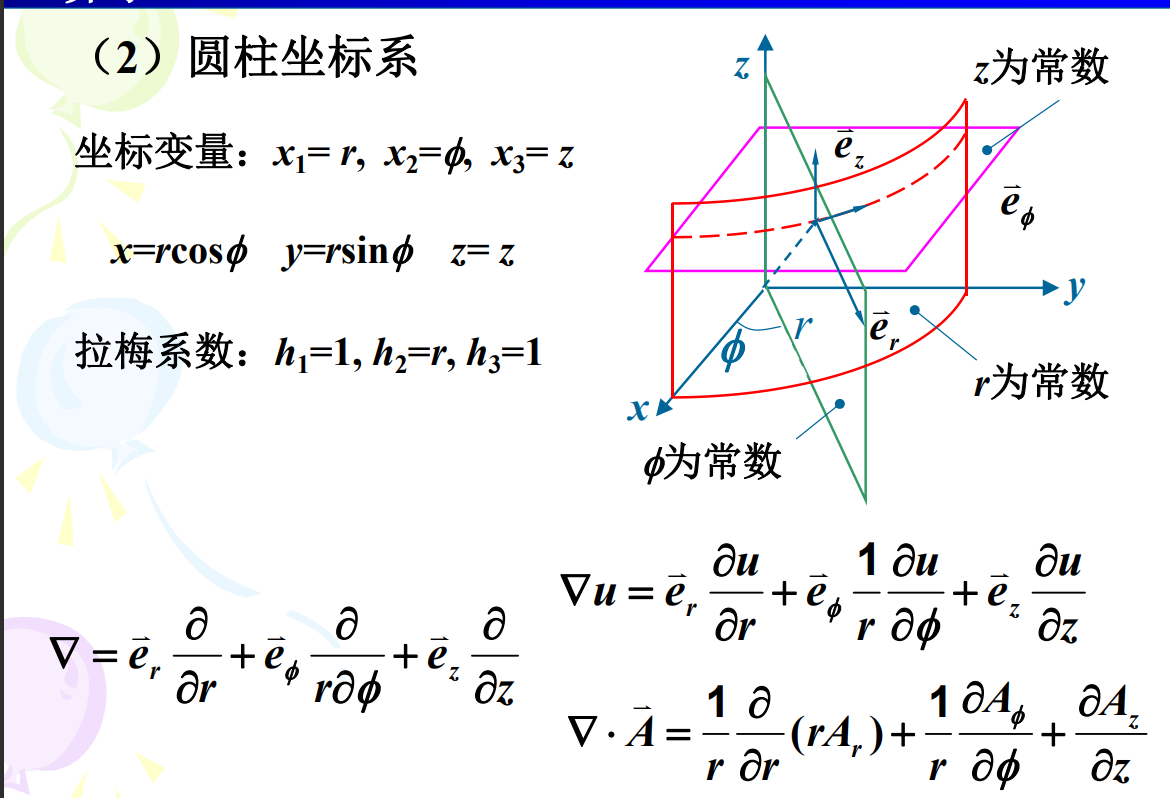
\includegraphics[width=7cm]{img/1.1.png}
        %     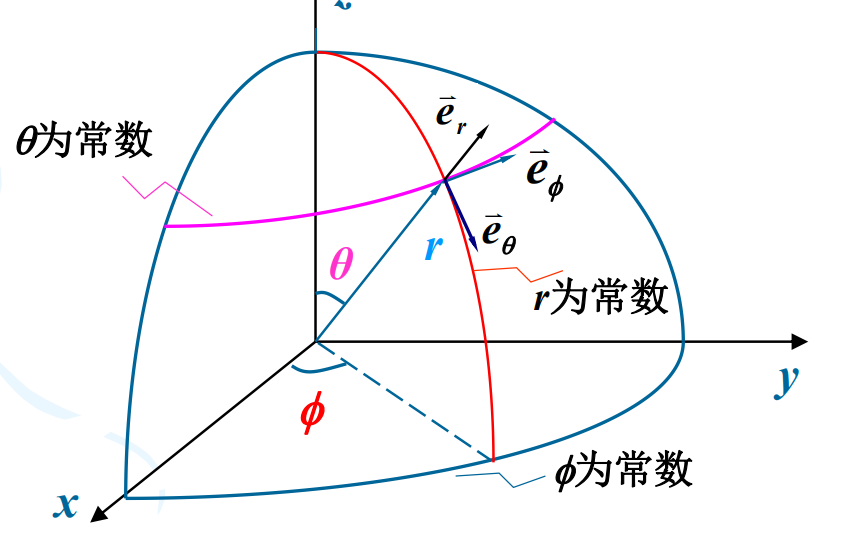
\includegraphics[width=7cm]{img/1.2.png}
        %     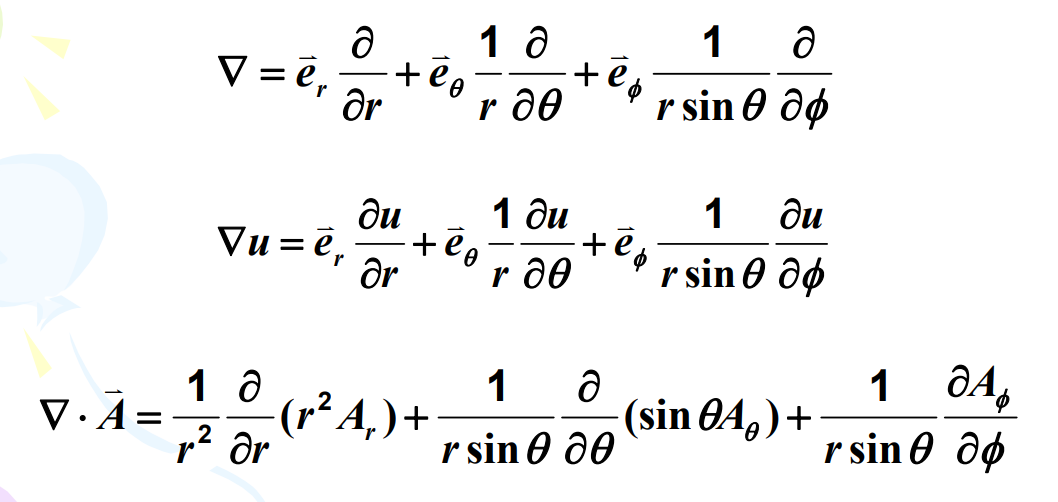
\includegraphics[width=7cm]{img/1.3.png}

        %     \end{figure}
        \subsection{并矢和张量}
\subsection{一些常用公式}
\subsubsection{源点场点}
\begin{equation}
\vec{r}=\vec{x}-\vec{x'}\tag{1.10}
\end{equation}
% 梯度
\begin{align}
\nabla r&= \frac{\vec{r}}{r}\tag{1.11.a} \\
\nabla' r &=-\frac{\vec{r}}{r}=-\nabla r\tag{1.11.a} \\
\nabla \cdot \vec{r}&=-\nabla'\vec{r}=3\tag{1.11.b} \\
\nabla \times \vec{r}&=\nabla'\times \vec{r}=0\tag{1.11.c} \\
\nabla f(u)&=\frac{\mathrm{d}{f}}{ \hspace{0.1cm} \mathrm{d}{u}}\nabla u \tag{1.11.d} \\ 
\nabla \cdot \vec{A}&=\nabla \cdot \frac{\mathrm{d}{\vec{A}}}{\mathrm{d}{u}}
\tag{1.11.e} 
\end{align}
% 散度

% 旋度
        \begin{figure}[H]
            \centering
            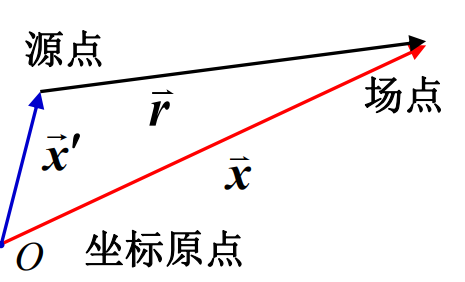
\includegraphics[width=7cm]{img/1.4.png}
            \end{figure}
\subsection{$\delta$函数}
\begin{equation}
  \int{}f(x)\delta(x-x_0)\mathrm{d}x \tag{1.12}
\end{equation}
$x_0$ 如果在积分范围里面就是$f(x_0)$,反之为0; 
\subsection{矢量场Helmholtz定理}
空间区域V上的任意矢量场,如果它的\underline{\textbf{散度}}、\underline{\textbf{旋度}}
和\underline{\textbf{边界条件}}已知,则该矢量场唯一确定,并可表示为无
散矢量场和无旋矢量场的叠加
\section{电磁现象}
\subsection{电场}
\begin{theorem}[库仑定律]
  \begin{equation}
  \vec{F}=\frac{qq'\vec{r}}{4 \pi \epsilon_0 r^3} \quad   \vec{F'}=-\vec{F}\tag{2.1}
  \end{equation}
\end{theorem}
\subsubsection{电场}
\begin{equation}
\tag{2.2}
\end{equation}
\subsubsection{高斯定律}
% \begin{equation}

% \end{equation}
\subsection{磁场}
\subsection{麦克斯韦方程组}
\subsection{介质的极化}
\subsubsection{极化电流}
\begin{align}
  \tag{3.1.a} \\

\end{align}
\end{document}